\documentclass[aspectratio=169]{beamer}
\usepackage{amsmath}
\usepackage{amssymb}
\usepackage{minted}
\usepackage{graphicx}
\title{Adaptive Envelope Rejection Sampling}
\subtitle{Applied to Log-concave Densities}
\author{Lucas Støjko Andersen}
\setminted{fontsize=\fontsize{8pt}{8pt}}
\institute{University of Copenhagen}
\date{\today}
\begin{document}
\begin{frame}
    \titlepage
\end{frame}
\begin{frame}
    \frametitle{Rejection Sampling}
    \framesubtitle{}
    Let $f, g$ be densities on $\mathbb{R}$ with $\alpha f\leq g$ for $\alpha > 0$. Let $U_{1},U_{2},\ldots$ be i.i.d. with uniform distribution and $Y_{1},Y_{2}\ldots$ be i.i.d. with density $g$ independent of the $U_{i}$'s. Define the stopping time
    \begin{equation}
      \sigma = \inf\{n\geq 1\mid U_{n}\leq\alpha f(Y_{n})/g(Y_{n})\}.
    \end{equation}
    Then $Y_{\sigma}$ has density $f$. The densities need not be normalized, however, if they are then $\alpha\in(0, 1]$ and $1 - \alpha$ is the probability of rejection.
\end{frame}
\begin{frame}[fragile]
  \frametitle{Rejection Sampling}
  \framesubtitle{Implementation}
\begin{minted}{r}
rejection_sampling <- function(n, 
                               density, 
                               env_density, 
                               env_sampler, 
                               alpha,
                               seed = NULL) {
  if(!is.null(seed)) set.seed(seed)
  samples <- numeric(n)
  succes <- tries <- 0
  for(s in 1:n) {
    reject <- TRUE
    while(reject) {
      tries <- tries + 1
      u0 <- runif(1)
      y0 <- env_sampler()
      env_y0 <- env_density(y0)
      dens_y0 <- density(y0)
      if(u0 <= alpha * dens_y0 / env_y0) {
        reject <- FALSE
        samples[s] <- y0
        succes <- succes + 1
      }
    }
  }
  list(samples, (tries - succes) / tries)
}
\end{minted}
\end{frame}
\begin{frame}[fragile]
  \frametitle{Rejection Sampling}
  \framesubtitle{Case Study}
  Let $f$ be the density with
  \begin{equation}
    f(y)\propto p(y)=\prod_{i=1}^{100}\exp(yz_{i}x_{i}-e^{yx_{i}}).
  \end{equation}
\begin{minted}{r}
poisreg <- function(x, z) {
  force(x); force(z)
  function(y) {
    expyx <- sapply(y, function(s) sum(exp(s * x)))
    exp(y * sum(x * z) - expyx)
  }
}
poisreg_derv <- function(x, z) {
  force(x)
  force(z)
  function(y) {
    expyx <- sapply(y, function(s) sum(exp(s * x)))
    x_expyx <- sapply(y, function(s) sum(x * exp(s * x)))
    xz <- sum(x * z) 
    exp(y * xz - expyx) * (xz - x_expyx)
  }
}
\end{minted}
\end{frame}
\begin{frame}
  \frametitle{Rejection Sampling}
  \framesubtitle{A Gaussian Envelope}
  The function $e^{(x - 0.2423914)^{2}/(2 \cdot 0.004079805)}$ is an envelope of $p$ with $\alpha = 1.351351\cdot 10^{40}$.
  \centering
  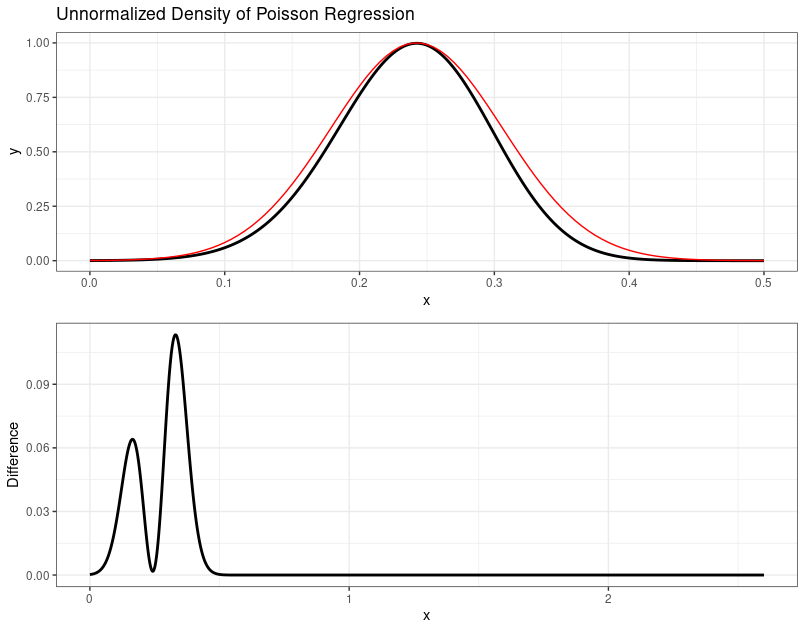
\includegraphics[scale = 0.4]{figure/GaussEnvelope.png}
\end{frame}
\begin{frame}[fragile]
  \frametitle{Adaptive Rejection Sampling}
\begin{minted}[fontsize = \fontsize{6.3pt}{6.3pt}]{r}
adap_samp <- function(n, density, density_deriv, p, zb = c(-Inf, Inf), seed = NULL) {
  if(!is.null(seed)) set.seed(seed)
  p <- sort(unique(p))
  densp <- density(p)
  a <- density_deriv(p) / densp
  b <- log(densp) - a * p
  a_diff <- a[-length(a)] - a[-1]
  check1 <- a[1] < 0 & zb[1] == -Inf
  check2 <- a[length(a)] > 0 & zb[2] == Inf
  if(check1 | check2)
    stop("Envelope is not integrable. Choose different points.")
  if(any(a == 0) | any(a_diff == 0))
    stop("Division by zero. Choose different points.")
  z <- c(zb[1], (b[-1] - b[-length(b)]) / a_diff, zb[2])
  env_quantile <- get_env_quantile(a, b, z)
  env_density <- get_env_density(a, b, z)
  samples <- numeric(n)
  succes <- tries <- 0
  for(s in 1:n) {
    reject <- TRUE
    while(reject) {
      tries <- tries + 1
      u0 <- runif(2)
      y0 <- env_quantile(u0[1])
      env_y0 <- env_density(y0)
      dens_y0 <- density(y0)
      if(u0[2] <= dens_y0 / env_y0) {
        reject <- FALSE
        succes <- succes + 1
        samples[s] <- y0
      }
    }
  }
  list(samples, (tries - succes) / tries)
}
\end{minted}
\end{frame}
\begin{frame}[fragile]
  \frametitle{Adaptive Rejection Sampling - Continued}
  \framesubtitle{Implementation}
\begin{minted}{r}
get_env_quantile<- function(a, b, z) {
  force(a); force(b); force(z)
  az <- a * z[-length(z)]
  R <- exp(b) * (exp(a * z[-1]) - exp(az)) / a
  Q1 <- numeric(length(a) + 1)
  Q1[2:length(Q1)] <- cumsum(R)
  c <- Q1[length(Q1)]
  function(q) {
    ind <- c * q <= Q1
    maxi <- which.max(ind) - 1
    y <- c * q - Q1[maxi]
    log(a[maxi] * y * exp(-b[maxi]) + exp(az[maxi])) / a[maxi]
  }
}

get_env_density <- function(a, b, z) {
  force(a); force(b); force(z)
  function(x) {
    if(x > z[length(z)] | x < z[1]) return(0)
    maxi <- which.max(x <= z) - 1
    exp(a[maxi] * x + b[maxi])
  }
}
\end{minted}
\end{frame}
\begin{frame}
  \frametitle{Comparison of the Implementations}
  \framesubtitle{}
  Simulating 100.000 samples with each implementation using the same seed. Using 0.15, 0.2, 0.28, 0.32 as the envelope points. The adaptive envelope had 0.09 rate of rejection and the gaussian envelope had 0.11 rate of rejection.
  \begin{figure}
  \centering
  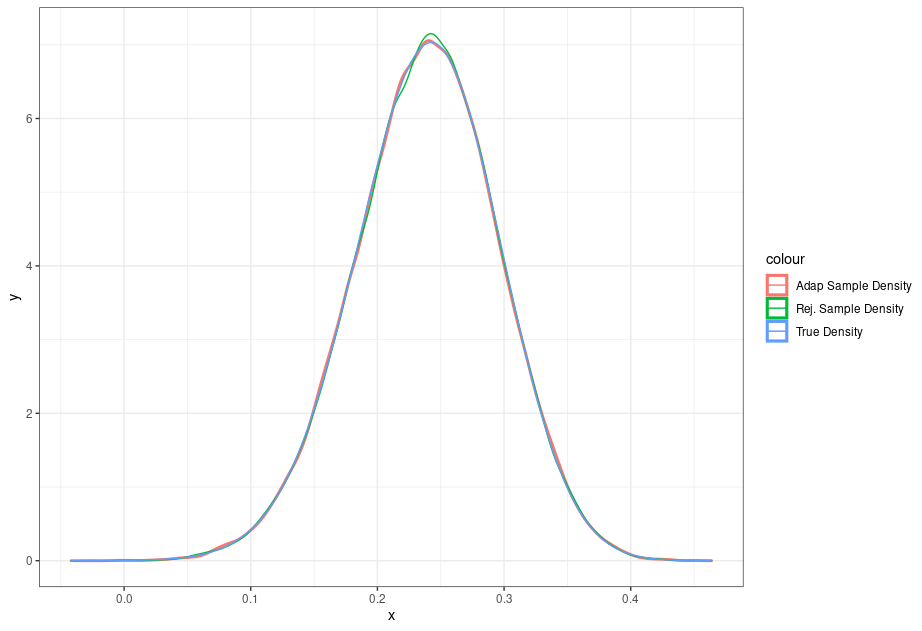
\includegraphics[scale = 0.36]{figure/AdapVsRejDensity.png}
  \end{figure}
\end{frame}
\begin{frame}
  \frametitle{Comparison of the Implementations}
  \framesubtitle{Benchmarks Using \texttt{bench} Package}
  Benchmarking sampling 100 samples.
  \begin{figure}
    \centering
    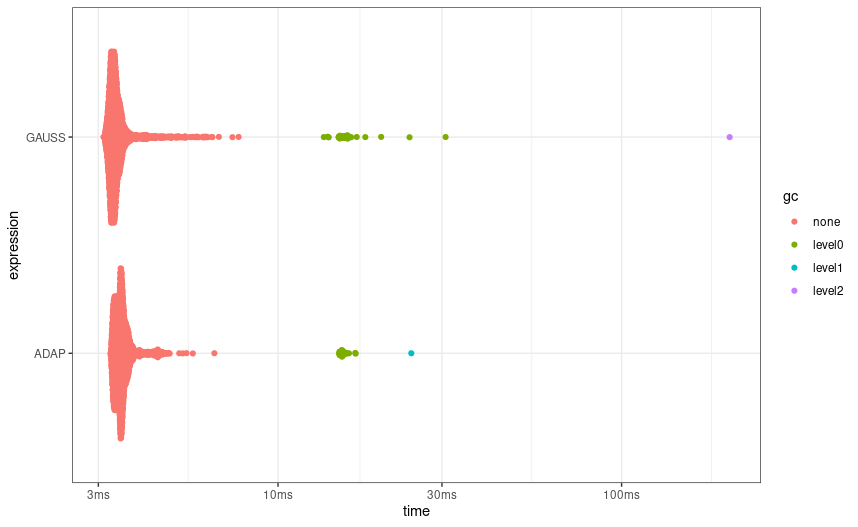
\includegraphics[scale = 0.4]{figure/GaussVsAdapPlot.png}
  \end{figure}
\end{frame}
\begin{frame}
  \frametitle{Comparison of the Implementations}
  \framesubtitle{Benchmarks Using \texttt{bench} Package}
  Benchmarking sampling 100 samples.
  \begin{figure}
    \centering
    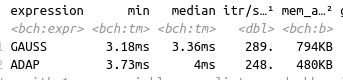
\includegraphics[scale = 0.6]{figure/AdapVsAdapTable.png}
  \end{figure}
\end{frame}
\begin{frame}
  \frametitle{Profiling the Implementation Using \texttt{profvis} Package}
  \centering
  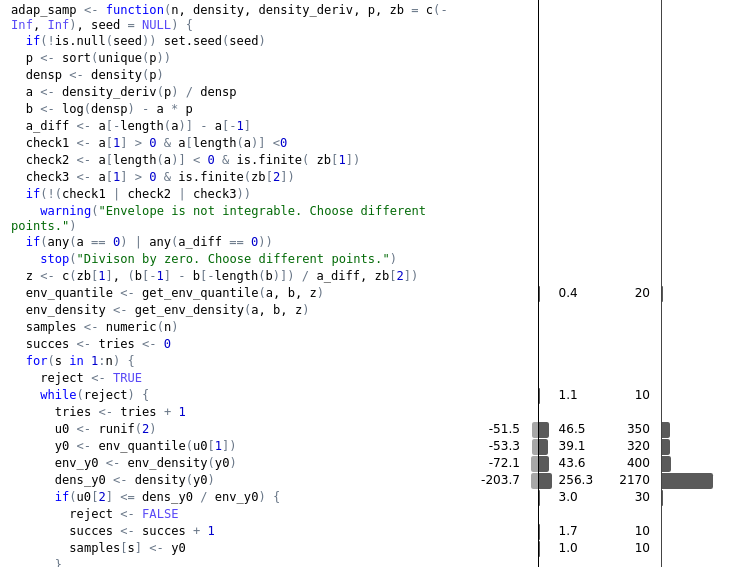
\includegraphics[scale = 0.4]{figure/ProfileBody.png}
\end{frame}
\begin{frame}
  \frametitle{Profiling the Implementation Using \texttt{profvis} Package}
  \centering
  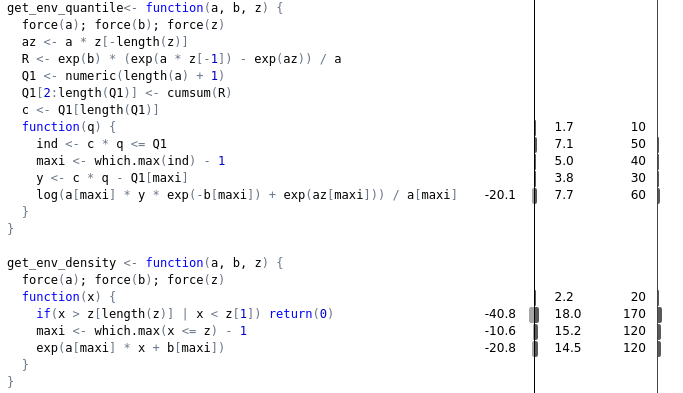
\includegraphics[scale = 0.4]{figure/ProfileHelper.png}
\end{frame}
\begin{frame}
  \frametitle{Profiling the Implementation Using \texttt{profvis} Package}
  \centering
  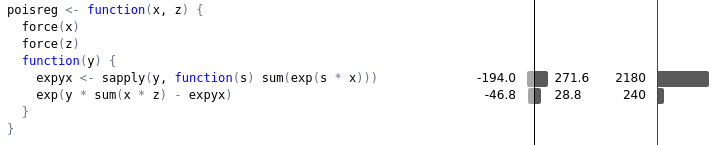
\includegraphics[scale = 0.5]{figure/ProfileLike.png}
\end{frame}
\begin{frame}[fragile]
  \frametitle{Improving the Implementation}
  \framesubtitle{Optimizing use of \texttt{runif}}  
\begin{minted}{r}
  u_samples <- runif(2 * n); k_stop <- n; k <- 1
  succes <- tries <- 0
  for(s in 1:n) {
    reject <- TRUE
    while(reject) {
      tries <- tries + 1
      if(k == k_stop) {
        u_samples <- runif(2 * (n - (s - 1)))
        k_stop <- n - (s - 1) + 1
        k <- 1
      }
      u0 <- u_samples[2 * (k - 1) + 1]
      u1 <- u_samples[2 * (k - 1) + 2]
      k <- k + 1
      y0 <- env_quantile(u0)
      env_y0 <- env_density(y0)
      dens_y0 <- density(y0)
      if(u1 <= dens_y0 / env_y0) {
        reject <- FALSE
        samples[s] <- y0
        succes <- succes + 1
      }
    }
  }
\end{minted}
\end{frame}
\begin{frame}[fragile]
  \frametitle{Improving the Implementation}
  \framesubtitle{Implementation of Envelope Quantile and Density Function in \texttt{RCPP}}  
\begin{minted}[fontsize = \fontsize{7pt}{7pt}]{cpp}
// [[Rcpp::export]]
double RCPP_env_density(double x, 
                        NumericVector a, 
                        NumericVector b, 
                        NumericVector z) {
  int m = z.size();
  if(x < z[0] || x > z[m - 1]) return 0;
  int maxi;
  for(maxi = 1; maxi < m; ++maxi)
    if(x <= z[maxi]) break;
  maxi -= 1;
  return std::exp(a[maxi] * x + b[maxi]);
}

// [[Rcpp::export]]
double RCPP_env_quantile(double x, 
                         NumericVector a, 
                         NumericVector b, 
                         NumericVector z,
                         NumericVector az,
                         NumericVector Q) {
  int m = Q.size(), maxi;
  double c = Q[m - 1];
  for(maxi = 0; maxi < m; ++maxi)
    if(c * x <= Q[maxi]) break;
  maxi -= 1;
  double y = c * x - Q[maxi];
  return std::log(a[maxi] * y * 
                  std::exp(-b[maxi]) + std::exp(az[maxi])) / a[maxi];
}
\end{minted}
\end{frame}
\begin{frame}[fragile]
  \frametitle{Improving the Implementation}
  \framesubtitle{Implementation of Envelope Quantile and Density Function in \texttt{RCPP}}
\begin{minted}{r}
get_env_quantile_cpp<- function(a, b, z) {
  force(a); force(b); force(z)
  az <- a * z[-length(z)]
  R <- exp(b) * (exp(a * z[-1]) - exp(az)) / a
  Q1 <- numeric(length(a) + 1)
  Q1[2:length(Q1)] <- cumsum(R)
  c <- Q1[length(Q1)]
  function(q) {
    RCPP_env_quantile(q, a, b, z, az, Q1)
  }
}

get_env_density_cpp <- function(a, b, z) {
  force(a); force(b); force(z)
  function(x) {
    RCPP_env_density(x, a, b, z)
  }
}
\end{minted}
\end{frame}
\begin{frame}
  \frametitle{Improving the Implementation}
  \framesubtitle{Benchmarking}
  \centering
  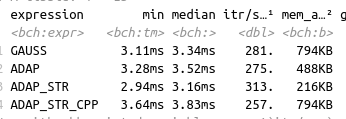
\includegraphics[scale = 0.6]{figure/RCPP_TABLE.png}
\end{frame}
\begin{frame}[fragile]
  \frametitle{Improving the Implementation}
  \framesubtitle{Partial \texttt{RCPP} Implementation}
\begin{columns}
\begin{column}{0.5\textwidth}
\begin{minted}[fontsize = \fontsize{6pt}{6pt}]{cpp}
// [[Rcpp::export]]
List RCPP_adap_samp_partial(int n,
                            Function density,
                            NumericVector a,
                            NumericVector b,
                            NumericVector z) {
  int m = a.size();
  std::vector<double> Q(m + 1);
  std::vector<double> az(m);
  Q[0] = 0;
  for(int i = 1; i < m + 1; ++i) {
    az[i - 1] = a[i - 1] * z[i - 1];
    Q[i] = Q[i - 1] + 
      std::exp(b[i - 1]) * 
      (std::exp(a[i - 1] * z[i]) - std::exp(az[i - 1])) / a[i - 1];
  }
\end{minted}
\end{column}
\begin{column}{0.5\textwidth}
\begin{minted}[fontsize = \fontsize{6pt}{6pt}]{cpp}





  NumericVector samples(n);
  int accepts = 0, tries = 0;
  for(int i = 0; i < n; ++i) {
    int reject = 1;
    while(reject == 1) {
      ++tries;
      double u0 = R::runif(0, 1);
      double u1 = R::runif(0, 1);
      double y0 = env_quantile(u0, a, b, az, Q);
      double env_y0 = env_density(y0, a, b, z);
      NumericVector dens_y0 = density(y0);
      if(u1 <= dens_y0[0] / env_y0) {
        reject = 0;
        samples[i] = y0;
        ++accepts;
      }
    }
  }
  NumericVector rate(1);
  rate[0] = ((double) tries - (double) accepts) / (double) tries;
  return List::create(samples, rate);
}
\end{minted}
\end{column}
\end{columns}
\end{frame}
\begin{frame}[fragile]
  \frametitle{Improving the Implementation}
  \framesubtitle{Partial \texttt{RCPP} Implementation}
\begin{minted}[fontsize = \fontsize{7pt}{7pt}]{cpp}
double env_quantile(double x,
                    NumericVector &a,
                    NumericVector &b,
                    std::vector<double> &az,
                    std::vector<double> &Q) {
  int n = a.size();
  double c = Q[n];
  int maxi;
  for(maxi = 0; maxi < n + 1; ++maxi)
    if(c * x <= Q[maxi]) break;
  maxi -= 1;
  double y = c * x - Q[maxi];
  return std::log(a[maxi] * y * std::exp(-b[maxi]) + 
                  std::exp(az[maxi])) / a[maxi];
}

double env_density(double x,
                   NumericVector &a,
                   NumericVector &b,
                   NumericVector &z) {
  int n = a.size();
  if(x > z[n] || x < z[0])
    return 0;
  int maxi;
  for(maxi = 0; maxi < n + 1; ++maxi)
    if(x <= z[maxi]) break;
  maxi -= 1;
  return std::exp(a[maxi] * x + b[maxi]);
}
\end{minted}
\end{frame}
\begin{frame}[fragile]
  \frametitle{Improving the Implementation}
  \framesubtitle{Partial \texttt{RCPP} Implementation}
\begin{minted}{r}
adap_samp_cpp_partial <- function(n, 
                                  density, 
                                  density_deriv, 
                                  p, 
                                  zb = c(-Inf, Inf),
                                  seed = NULL) {
  if(!is.null(seed)) set.seed(seed)
  p <- sort(unique(p))
  densp <- density(p)
  a <- density_deriv(p) / densp
  b <- log(densp) - a * p
  a_diff <- a[-length(a)] - a[-1]
  check1 <- a[1] < 0 & zb[1] == -Inf
  check2 <- a[length(a)] > 0 & zb[2] == Inf
  if(check1 | check2)
    stop("Envelope is not integrable. Choose different points.")
  if(any(a == 0) | any(a_diff == 0))
    stop("Divison by zero. Choose different points.")
  z <- c(zb[1], (b[-1] - b[-length(b)]) / a_diff, zb[2])
  
  RCPP_adap_samp_partial(n, density, a, b ,z)
}
\end{minted}
\end{frame}
\begin{frame}
  \frametitle{Improving the Implementation}
  \framesubtitle{Benchmark}
  \centering
  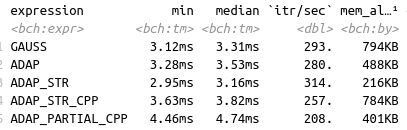
\includegraphics[scale = 0.6]{figure/RCPP_FULL.png}
\end{frame}
\begin{frame}[fragile]
  \frametitle{Implementing Adaptive Envelope Sampling Using \texttt{R}'s C API}
\begin{columns}
\begin{column}{0.5\textwidth}
\vspace*{-1.5cm}
\begin{minted}[fontsize = \fontsize{6pt}{6pt}]{c}
#include <R.h>
#include <math.h>
#include <Rinternals.h>
#include <R_ext/Random.h> // ACCESS TO UNIF NUMBER GENERATOR

SEXP C_adap_samp(SEXP n,
                 SEXP density,
                 SEXP a,
                 SEXP b,
                 SEXP z,
                 SEXP rho) {
  int m = length(a);
  int N = INTEGER(n)[0];
  double *Q = (double *)malloc(sizeof(double) * (m + 1));
  double *az = (double *)malloc(sizeof(double) * m);
  double *a_ = REAL(a), *b_ = REAL(b), *z_ = REAL(z);

  Q[0] = 0;
  for(int i = 1; i < m + 1; ++i) {
    az[i - 1] = a_[i - 1] * z_[i - 1];
    Q[i] = Q[i - 1] + 
      exp(b_[i - 1]) * (exp(a_[i - 1] * z_[i]) - exp(az[i - 1])) / 
      a_[i - 1];
  }
\end{minted}
\end{column}
\begin{column}{0.5\textwidth}
\begin{minted}[fontsize = \fontsize{5.7pt}{5.7pt}]{c}
  SEXP density_call = PROTECT(lang2(density, R_NilValue));
  SEXP samples = PROTECT(allocVector(REALSXP, N));
  double *samples_ = REAL(samples);
  int accepts = 0, tries = 0;
  GetRNGstate();
  for(int i = 0; i < N; ++i) {
    int reject = 1;
    while(reject == 1) {
      ++tries;
      double u0 = unif_rand();
      double u1 = unif_rand();
      double y0 = env_quantile(u0, a_, b_, az, Q, m);
      double env_y0 = env_density(y0, a_, b_, z_, m);
      SETCADR(density_call, PROTECT(ScalarReal(y0)));
      SEXP dens_y0 = eval(density_call, rho);
      UNPROTECT(1);
      if(u1 <= REAL(dens_y0)[0] / env_y0) {
        reject = 0;
        samples_[i] = y0;
        ++accepts;
      }
    }
  }
  PutRNGstate();
  SEXP values = PROTECT(allocVector(VECSXP, 2));
  double rate = ((double) tries - (double) accepts) / (double) tries;
  SET_VECTOR_ELT(values, 0, samples);
  SET_VECTOR_ELT(values, 1, ScalarReal(rate));
  UNPROTECT(3);
  free(Q);
  free(az);
  return values;
}
\end{minted}
\end{column}
\end{columns}
\end{frame}
\begin{frame}[fragile]
  \frametitle{Implementing Adaptive Envelope Sampling Using \texttt{R}'s C API}
\begin{minted}{c}
double env_quantile(double x,
                    double *a,
                    double *b,
                    double *az,
                    double *Q,
                    int n) {
  double c = Q[n];
  int maxi;
  for(maxi = 0; maxi < n + 1; ++maxi)
    if(c * x <= Q[maxi]) break;
  maxi -= 1;
  double y = c * x - Q[maxi];
  return log(a[maxi] * y * exp(-b[maxi]) + exp(az[maxi])) / a[maxi];
}

double env_density(double x,
                   double *a,
                   double *b,
                   double *z,
                   int n) {
  if(x > z[n] || x < z[0])
    return 0;
  int maxi;
  for(maxi = 0; maxi < n + 1; ++maxi)
    if(x <= z[maxi]) break;
  maxi -= 1;
  return exp(a[maxi] * x + b[maxi]);
}
\end{minted}
\end{frame}
\begin{frame}[fragile]
  \frametitle{Implementing Adaptive Envelope Sampling Using \texttt{R}'s C API}
\begin{minted}{r}
adap_samp_c <- function(n, density, density_deriv, p, seed = NULL, zb = c(-Inf, Inf)) {
  if(!is.null(seed)) set.seed(seed)
  p <- sort(unique(p))
  densp <- density(p)
  a <- density_deriv(p) / densp
  b <- log(densp) - a * p
  a_diff <- a[-length(a)] - a[-1]
  check1 <- a[1] < 0 & zb[1] == -Inf
  check2 <- a[length(a)] > 0 & zb[2] == Inf
  if(check1 | check2)
    stop("Envelope is not integrable. Choose different points.")
  if(any(a == 0) | any(a_diff == 0))
    stop("Divison by zero. Choose different points.")
  z <- c(zb[1], (b[-1] - b[-length(b)]) / a_diff, zb[2])
  
  .Call("C_adap_samp",
        as.integer(n),
        density,
        a,
        b,
        z,
        environment())
}
\end{minted}
\end{frame}
\begin{frame}
  \frametitle{Final Benchmarks}
  \framesubtitle{Table}
  \centering
  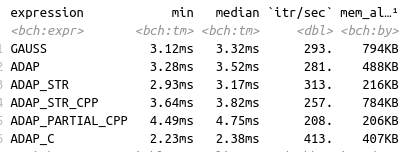
\includegraphics[scale = 0.5]{figure/C_TABLE.png}
\end{frame}
\begin{frame}
  \frametitle{Final Benchmarks}
  \framesubtitle{Scaling}
  \centering
  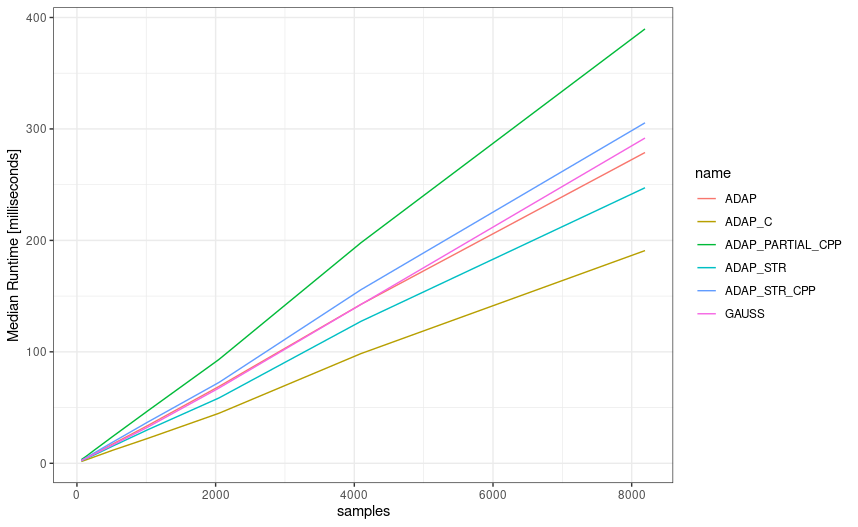
\includegraphics[scale = 0.5]{figure/MedianRuntime.png}
\end{frame}
\begin{frame}
  \frametitle{Final Benchmarks}
  \framesubtitle{Scaling}
  Different points 0.1, 0.2, 0.3 for adaptive envelope.
  \centering
  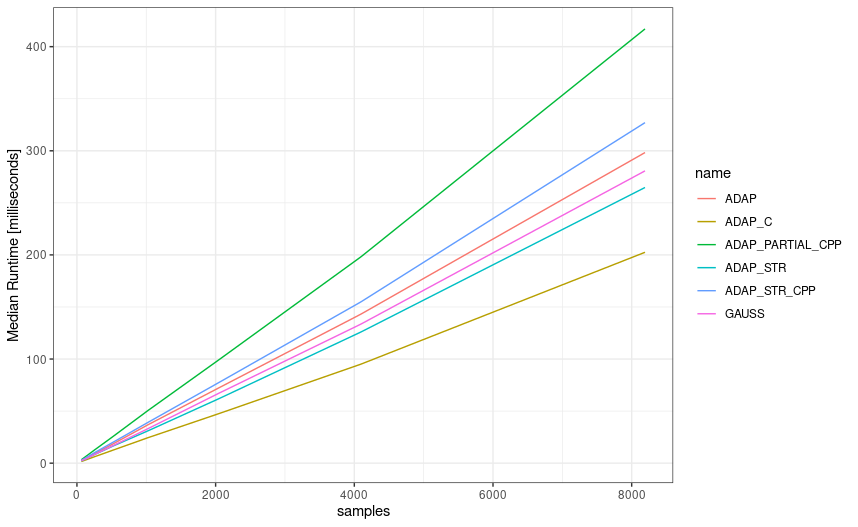
\includegraphics[scale = 0.45]{figure/MedianRuntime2.png}
\end{frame}
\begin{frame}
  \frametitle{Density of Samples from C Implementation}
  \centering
  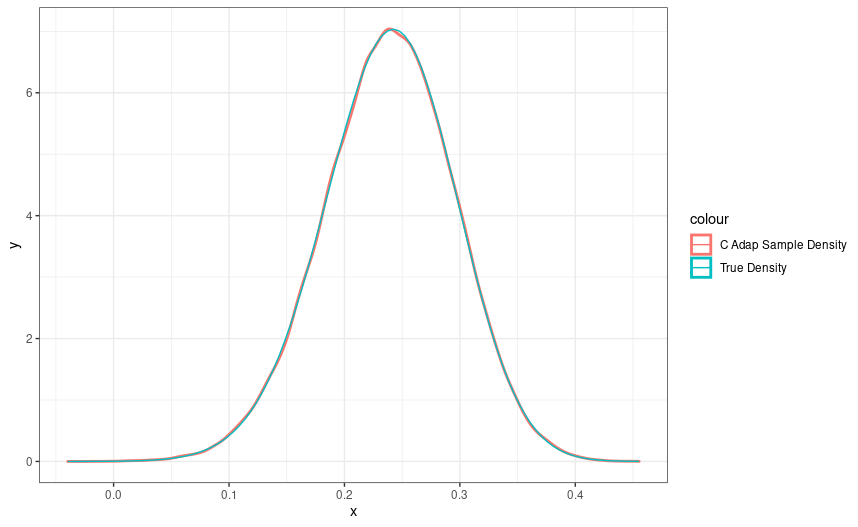
\includegraphics[scale = 0.45]{figure/CAdapDensity.png}
\end{frame}
\end{document}
